\documentclass[final]{beamer}
\mode<presentation>
{
  \usetheme{I6pd2}
}
\graphicspath{{figures/}} % e.g. where you have your logos

\usepackage{epstopdf}
\usepackage{times}
\usepackage{amsmath,amssymb}
\usepackage[english]{babel}
\usepackage[latin1]{inputenc}
\usepackage{ragged2e} 
\usepackage{multicol}
\usepackage{tabularx}
\usepackage{changepage}

\addtobeamertemplate{block begin}
  {}
  {
   \begin{adjustwidth}{1cm}{1cm}
}
\addtobeamertemplate{block end}
  {\end{adjustwidth}}% Pads bottom of block

\setbeamertemplate{bibliography item}[text]

\usepackage[orientation=portrait, size=a0, scale=1.4, debug]{beamerposter} 
\title[Fancy Posters]{REXOS}
\author{Daniel Telgen et al.}

\institute{HU University of Applied Sciences Utrecht}
\date{\today}

\newcommand{\columnblock}[2][Title]{
    \begin{block}{\large \vspace{-0.5cm}#1}
    #2
    \end{block}
}

\newcommand{\twocolumnsblock}[3][Title]{
    \columnblock[#1]{
        \begin{multicols}{2}
            #2
            \newpage
            #3
        \end{multicols}
    }
}

\begin{document}


\begin{frame}{}
	\columnblock[Architecture]{
		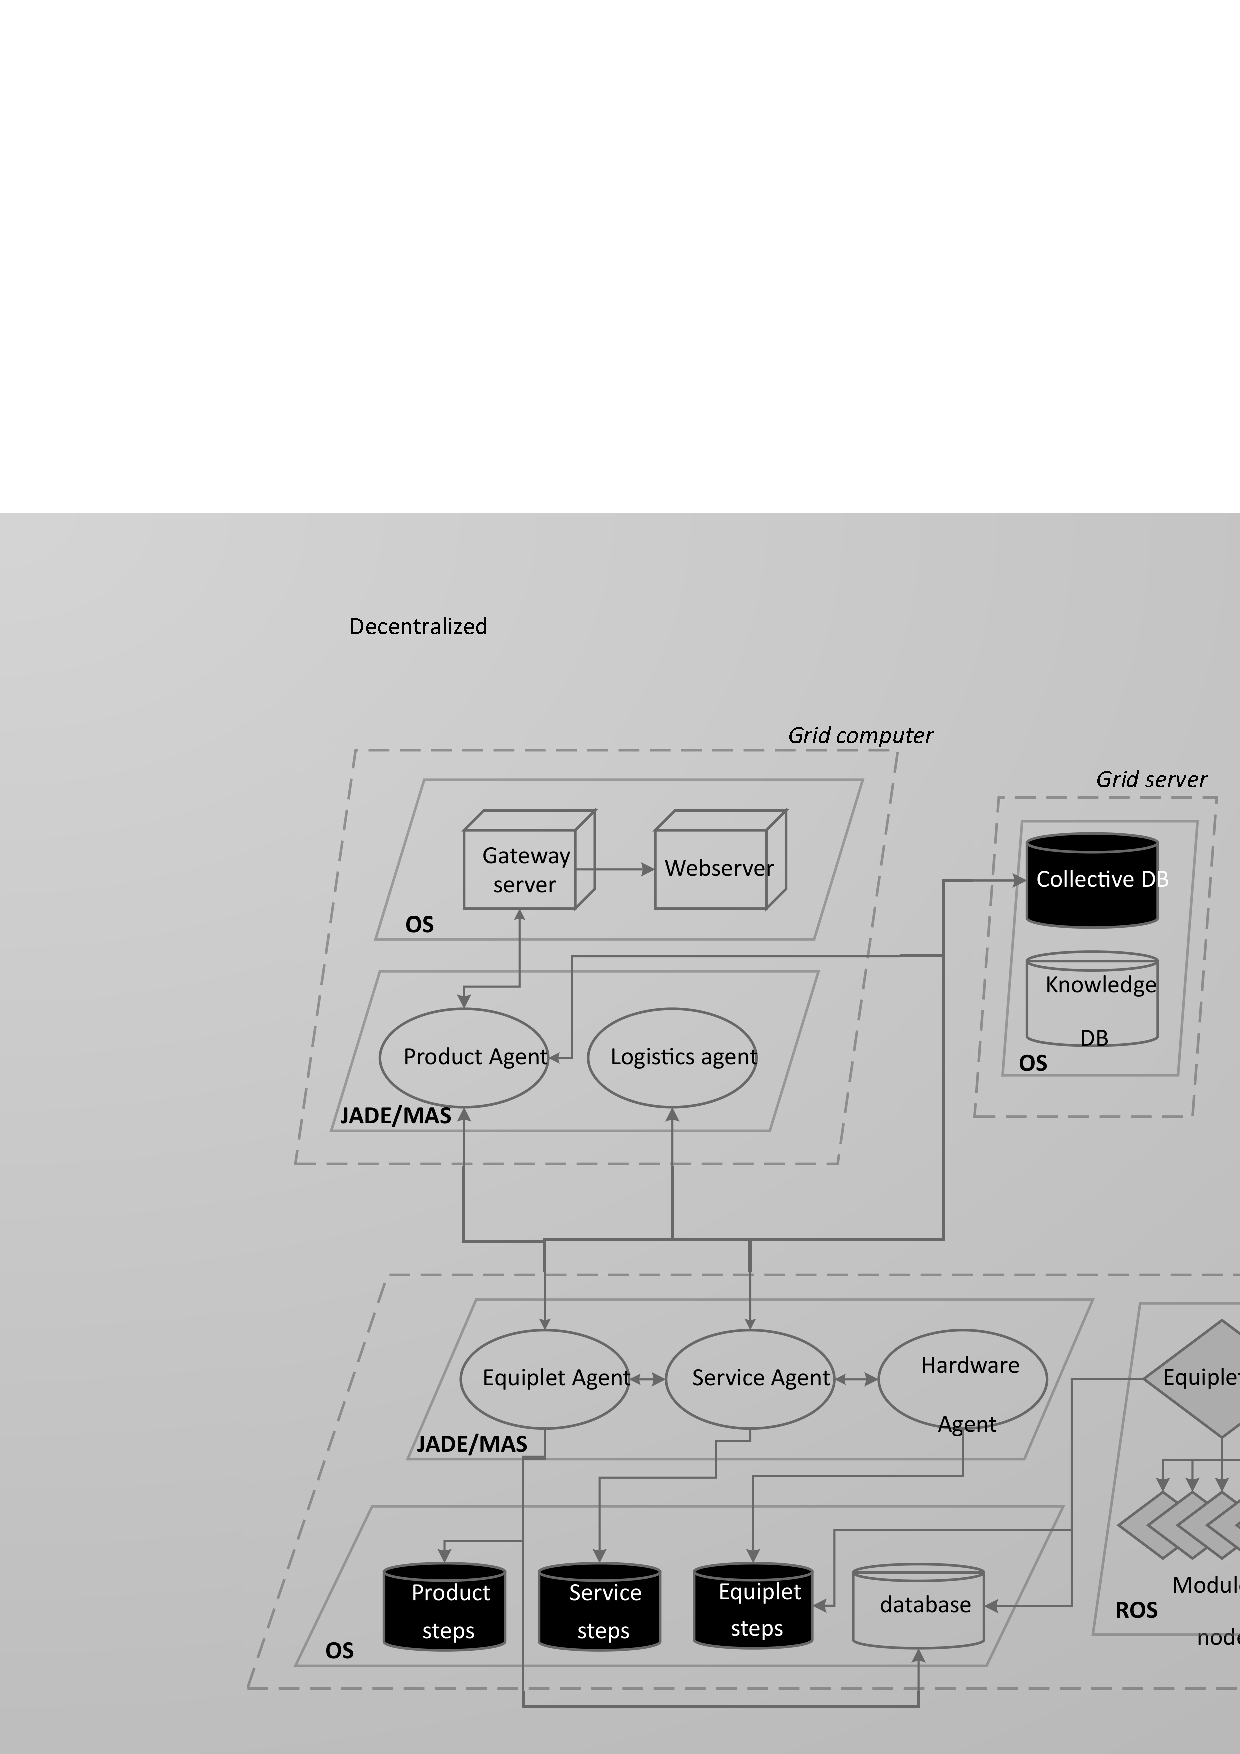
\includegraphics[trim= 9cm 0cm 9cm 0cm, clip=true, width=.98\linewidth] {Decentralized_REXOS}
	}
	
    \begin{columns}[t]   
		\begin{column}{.48\textwidth}
	        % == Introduction == %        
            \columnblock[Introduction]{
            \justifying
            Advances in technology and business strategy have brought manufacturing paradigms such as Agile Manufacturing (AM) and Reconfigurable Manufacturing Systems (RMS). The key of both paradigms is flexibility. This results in the user being able to produce a high mix of products with low amounts produced. There are many technical challenges that require research to be overcome. By utilizing agent technology, we try to overcome these challenges. This has led to a new hybrid control architecture which combines both the intelligence and structure of autonomous multi-agent systems (MAS) and the flexibility of Robot Operating Systems (ROS). We have called this REXOS. 

            }
            
            
            % == Grid == %
            \columnblock[Grid]{
            \justifying 
            Grids consist of multiple equiplets manufacturing in parallel. All the equiplets in the grid are autonomous systems, however, when they are combined, a greater variety of products can be produced. Due to the highly reconfigurable nature of Equiplets and the grid in general, grid refinement for manufacturing can be achieved on a daily basis.
            \includegraphics[ trim= 2cm 0cm 1cm 0cm, clip=true, width=1\linewidth]{Grid}
            }
            
             
            
		\end{column}		
		% ====== END OF COLUMN A ====== %

		% ====== START OF COLUMN B ===== %        
		\begin{column}{.48\textwidth}
            \columnblock[REXOS]{
            \justifying 
REXOS is a hybrid system consisting of a reactive layer and a deliberating layer. In terms of manufacturing, the reactive layer resembles the control of the hardware on the equiplets while the deliberating layer resembles the decision making part of the production itself ( i.e. scheduling, choosing equiplets to produce on and transportation decisions ). This layer needs to make intelligent and cognitive decisions. The reactive layer consists of nodes running on a ROS platform. The deliberating layer consists of agents running on a JADE platform. These layers need to communicate with each other. To accomplish this, a third layer, the communication layer, is added. This layer uses blackboards to accomplish this. equiplets within the REXOS architecture can run individually or within a grid of Equiplets. 
            }
            
            % == Equiplet == %
            \twocolumnsblock[Equiplet]{
            \justifying 
            An equiplet is a generic modular machine used for agile and sustainable manufacturing. Equiplets are designed to be low cost and easy to configure. Equiplets can easily be reconfigured by scanning QR codes in order to add or remove modules. The agent system can load the required (control) software and calibrate its own systems. Equiplets are able to act autonomously and are also able to work together in a grid. On their own, a single eequiplet provides one service with limited capability. However, a group of equiplets can offer a large range of services and can easily be customized for the current demand.
            {\includegraphics[width=0.95\linewidth]{equiplets.png}}
            }
                        
                  
		\end{column}
    \end{columns}    
\end{frame}
\end{document}